\section{Experiments}
\label{sec:experiments}

This section describes the experiments we conducted to evaluate our and third 
party implementation of the Multinomial Naive Bayes models and respective 
semi-supervised extensions described in Section~\ref{sec:methodology}.

\subsection{Experimental Setup}
\label{subsec:exp-setup}

We start with a brief description of the dataset used in our experiments, 
followed by the plan of experiments whose results are shown 
in Section~\ref{subsec:exp-res}.

\subsubsection{Dataset}
\label{subsubsec:dataset}

We work with the 20 Newsgroups dataset~\cite{Lang95}, which consists in a 
collection of approx. 19000 web forum posts, (almost) evenly separated 
across 20 different topics~\footnote{A list of topics is available in \url{http://qwone.com/~jason/20Newsgroups/}.}. 
Although separated from each other, some of the 20 classes are related to each other as sub-topics of a larger 
category (e.g. \verb+rec.sport.baseball+ and \verb+rec.sport.baseball+ as 
sub-topics of \verb+rec.sport.*+). The posts were collected over a period 
of several months in 1993~\cite{Nigam2000}.\vertbreak 

For our 
experiments, we consider a modified version of the \verb+20news-bydate+ 
dataset~\footnote{Available in \url{http://qwone.com/~jason/20Newsgroups/}.}. 
The \verb+20news-bydate+ provides a dataset 
sorted by date, with separate training and test subsets (test subset composed by later posts), comprising a total of 
18846 newsgroups articles. 
Using the Rainbow tools~\cprotect\footnote{Available in \url{http://www.cs.cmu.edu/~mccallum/bow/rainbow/}. Due to compiling issues with the original versions 
of Rainbow, we have used the following patched version which compiles 
with \verb+gcc+ version 4.6.3: \url{https://github.com/brendano/bow/}.}, developed by the authors of~\cite{McCallum98acomparison,Nigam2000}, we have 
modified the dataset to (1) remove newsgroups headers (a common practice since 
the article headers include the name of the newsgroup they belong to, which 
would make classification trivial), (2) remove 524 common `stop words' (e.g. 
`the', `of') and (3) remove words which occur only 1 time. These feature 
selection approaches are made 
in previous works on text 
classification~\cite{McCallum98acomparison,Nigam2000,Kibriya:2004:MNB:2146834.2146882,Su2011} and are mainly used as 
attempts to reduce the data dimensionality (i.e. size of the dictionary, 
$|\mathcal{D}|$. We have noticed that (2) was necessary to achieve similar MNB 
accuracies to those reported in~\cite{McCallum98acomparison,Nigam2000}. The characteristics of the modified 
\verb+20news-bydate+ are summarized in Table~\ref{tab:dataset-chars}.

\begin{table}
    \begin{center}
        \begin{tabular}{|l|c|c|}
            \hline
            \textbf{Partition}   & \textbf{\# Articles}   & \textbf{\# Unique Words} \\
            \hline\hline
            Training    & 11260         & 53485 \\
            Test        & 7502          & 60698 \\
            \hline
        \end{tabular}
    \end{center}
    \cprotect\caption{Characteristics of version of \verb+20news-bydate+ dataset used in experiments.}
    \label{tab:dataset-chars}
\end{table}

\subsubsection{Experimental Protocol}
\label{subsubsec:protocol}

The protocol is structured to test the different methods presented in 
Section~\ref{sec:methodology}, in the same order.\vertbreak

\textbf{A) Multinomial Naive Bayes}\vertbreak

We test our implementation of the MNB classifier, together with Rainbow's, 
evaluating accuracy and confusion between actual and predicted classifications 
under different conditions. We evaluate total and per-class accuracy $Acc$ in 
\%, according to expression~\ref{eq:acc}:

\begin{equation}
    Acc = \frac{\text{\# correctly classified articles}}{\text{total \# classified articles}}
    \label{eq:acc}
\end{equation}

The MNB classifiers are tested over the test set (see 
Table~\ref{tab:dataset-chars}), for different sample sizes 
$|\mathcal{A}^{\ell}| = \{20, 50, 100, 500, 1000, 5000, 7520\}$ from the training set. 
For each case, we randomly sample $|\mathcal{A}^{\ell}| / 20$ articles 
from each of the 20 topics and show the average results over 20 runs of this procedure.\vertbreak

\textbf{B) Multinomial Naive Bayes + EM}\vertbreak

We test our implementation of the MNB + EM combination, together with Rainbow's, 
again evaluating accuracy and confusion between actual and predicted classifications 
under different conditions. The selection of $\mathcal{A}^{\ell}$ and 
$\mathcal{A}^{u}$ sets is done as follows:

\begin{enumerate}

    \item We first select a $\mathcal{A}^{\ell}$ sample of size 
        $|\mathcal{A}^{\ell}| = \{20, 40, 100, 300, 500, 800, 1000, 1260\}$ from 
        the training subset, again $|\mathcal{A}^{\ell}| / 20$ articles 
        from each of the 20 topics.
    \item We use the remaining $11260 - |\mathcal{A}^{\ell}|$ as unlabeled 
        data $\mathcal{A}^{u}$.

\end{enumerate}

The values of $|\mathcal{A}^{\ell}|$ are chosen so that 
$|\mathcal{A}^{u} \ge 10000|$, for comparison with the results from~\cite{Nigam2000}. 
Again, we show the average results over 20 runs of this procedure. As a 
baseline for direct comparison we use the 
results for the fully supervised MNB classifier, trained with each different 
$\mathcal{A}^{\ell}$ set.\vertbreak

\textbf{C) Multinomial Naive Bayes + EM-$\lambda$}\vertbreak

We test our implementation of the MNB + EM-$\lambda$ combination, in a similar 
way to that of the basic EM case. Here we additionally test several values of 
$\lambda = \{0.01, 0.02, 0.1, 0.2, 0.5, 1.0\}$, evaluating accuracy and confusion 
between actual and predicted classifications.

\subsection{Experimental Results}
\label{subsec:exp-res}

We present the results for the experiments described in the previous section. 
Due to problems with our implementation of EM and 
EM-$\lambda$\,\footnote{Errors in the M-step of the EM algorithm. The code 
is available in \url{http://paginas.fe.up.pt/~up200400437/mlproject.zip} for 
reference}, we only compare 
our implementation of MNB in MATLAB to that of the Rainbow 
framework. Nevertheless, we provide the results obtained with Rainbow, using 
the modified version of the \verb+20news-bydate+ dataset.\vertbreak

In Figure~\ref{fig:mnb} we present the results of the supervised MNB 
classifier. The accuracy values for the Rainbow's version closely follow those 
reported in~\cite{Nigam2000}. For low values of $|A^\ell|$, our implementation 
of MNB (which follows the methodology provided in Section~\ref{subsec:multinomial-naive}) provides 
worse results than Rainbow's, with closer values for $|A^\ell| > 5000$.\vertbreak

\begin{figure}[h!]

    \centering
    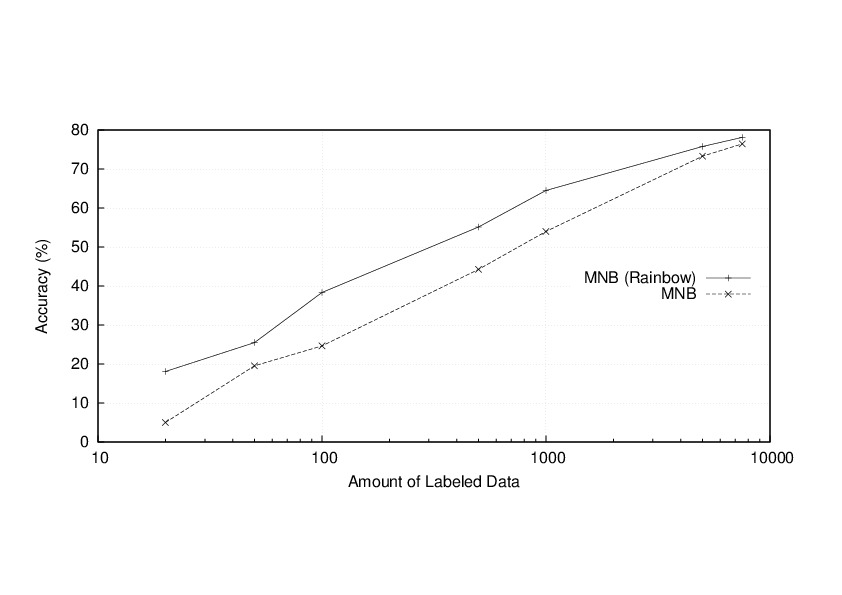
\includegraphics[width=0.40\textwidth]{figures/mnb.pdf}
    \cprotect\caption{Results for test A: MNB, using Rainbow's framework and 
        our implementation in MATLAB.}
    \label{fig:mnb}

\end{figure}

The results for test B, shown in Figure~\ref{fig:mnb-em}, partly reproduce the 
results found in~\cite{Nigam2000}, since for the lower $|A^\ell|$ the average 
results of MNB + EM surpass those for MNB. For $|A^\ell| > 40$, MNB provides 
better accuracies, nevertheless one should 
note we use a larger testing set (7502 vs. 4000) and a different method 
for choosing $A^\ell$ and $A^u$. MNB + EM accuracy strongly varies during 
the 20 runs, consistently providing higher maximums and lower minimums than 
MNB, for all $|A^\ell|$ (see Figure~\ref{fig:mnb-em-max-min}). The maximum values 
for MNB + EM approach those reported in~\cite{Nigam2000}. 
Figures~\ref{fig:mnb-em-mnb} and~\ref{fig:mnb-em-em} show four cases of 
confusion matrices for test B, $A^\ell = 1260$, for both MNB and MNB + EM 
methods. One can clearly verify EM's clustering nature on the right side of 
Figure~\ref{fig:mnb-em-max-min}, with a significant number of false predictions 
for articles belonging to \verb+comp.*+ subgroups, mostly classified as 
belonging to the class \verb+comp.graphics+. As expected, the main focus of 
confusion occur for clusters of subgroups, namely \verb+comp.*+, \verb+sci.*+ (with a considerable 
number of articles belonging to several \verb+comp.*+ subgroups being misclassified 
as \verb+sci.crypt+) and \verb+talk.*+, for both MNB and MNB + EM cases.

\begin{figure}[h!]

    \centering
    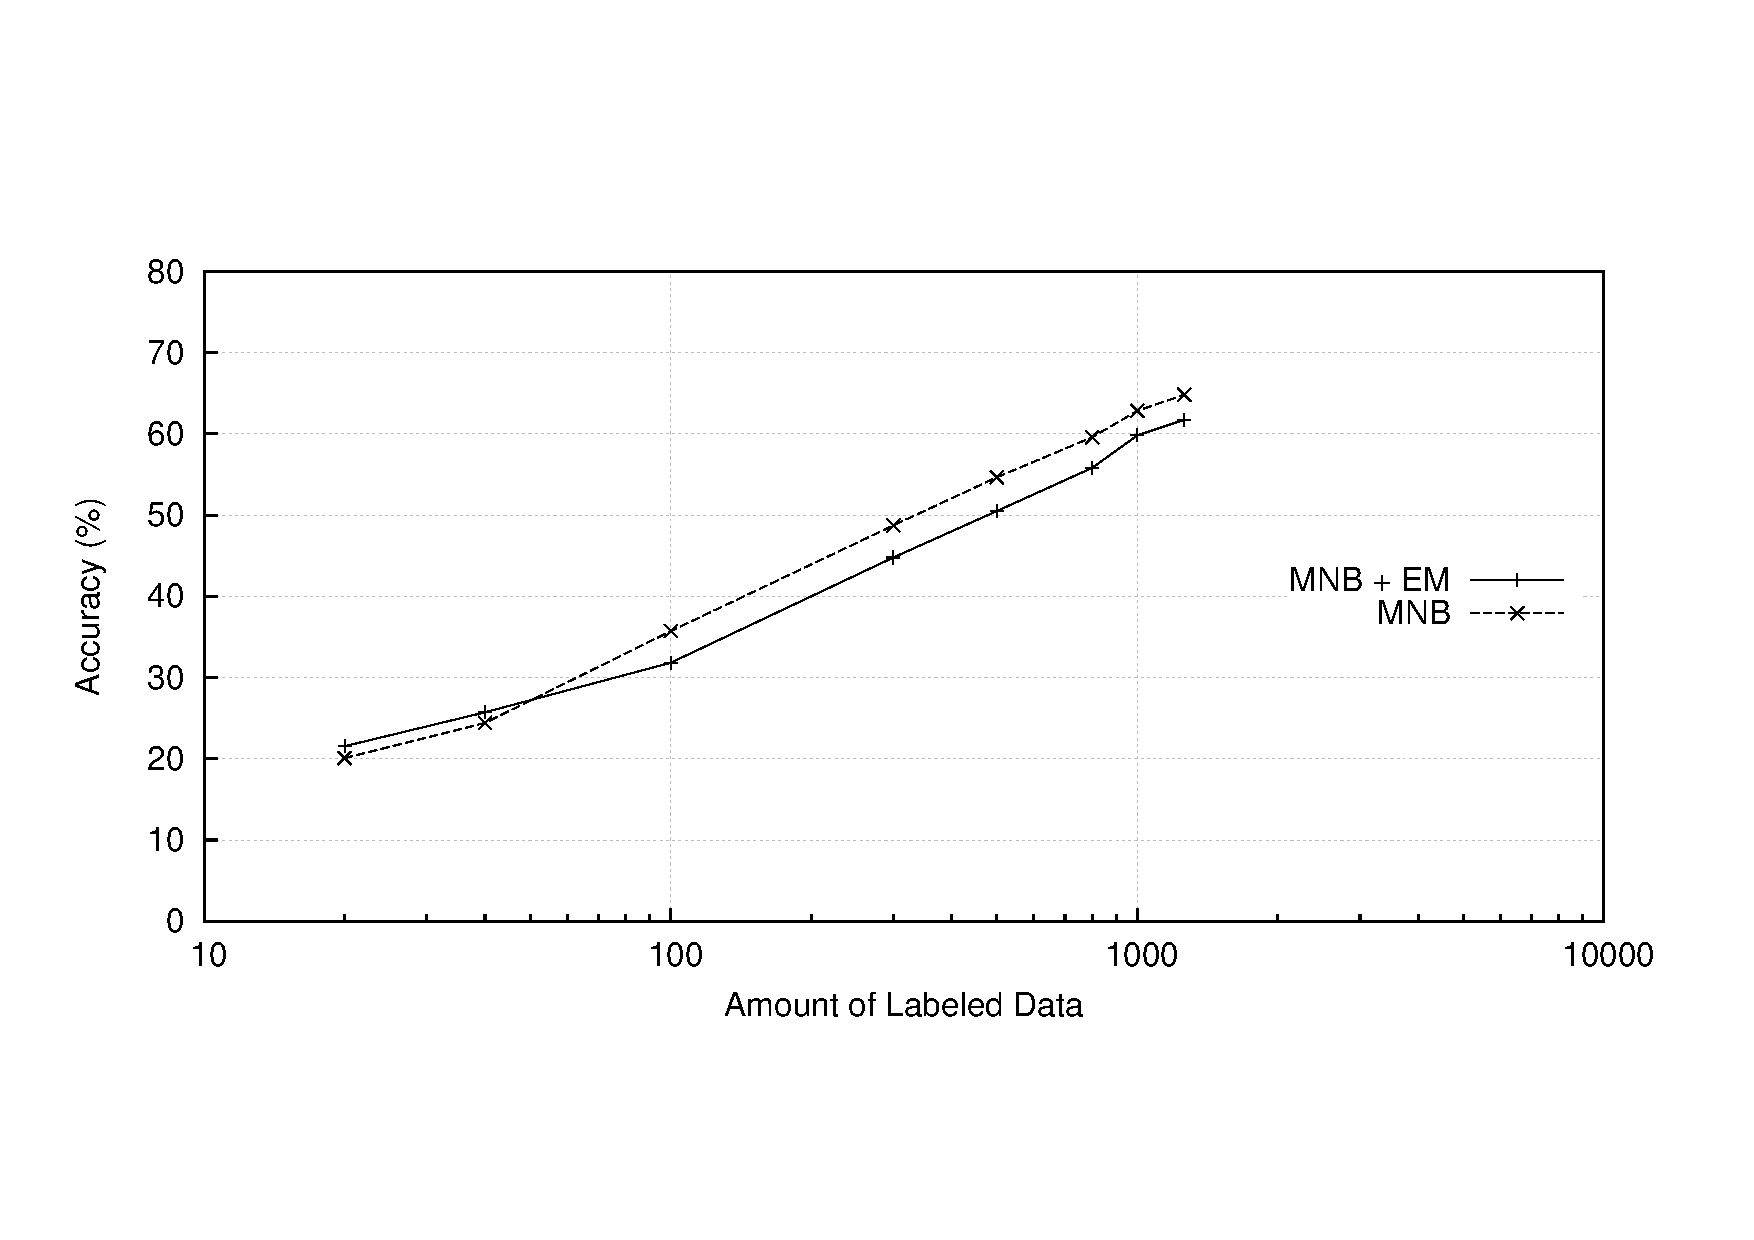
\includegraphics[width=0.40\textwidth]{figures/em.pdf}
    \cprotect\caption{Results for test B: MNB + EM, using Rainbow's framework. 
        The results of MNB for the same $A^\ell$ are also given.}
    \label{fig:mnb-em}

\end{figure}

\begin{figure}[h!]

    \centering
    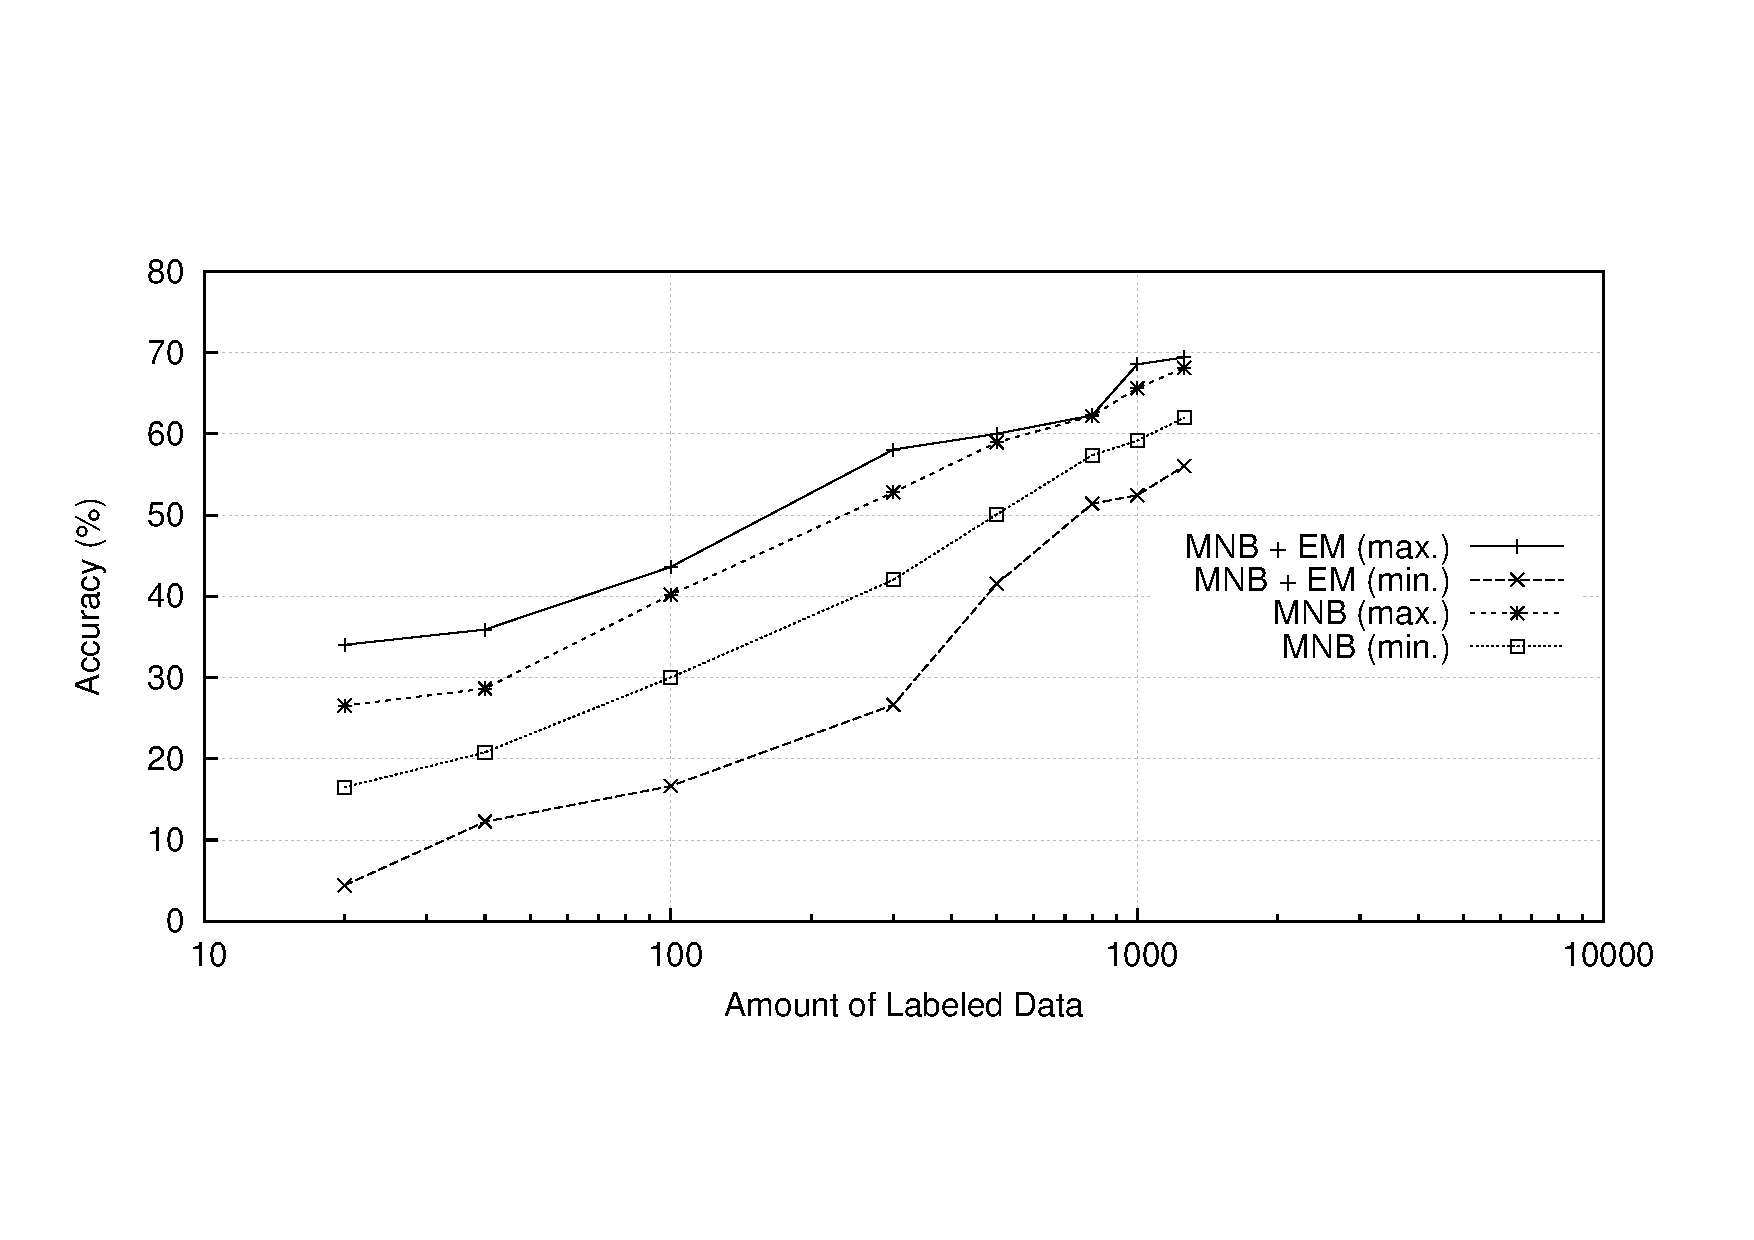
\includegraphics[width=0.40\textwidth]{figures/em-max-min.pdf}
    \cprotect\caption{Results for test B: MNB + EM, using Rainbow's framework. 
        The results of MNB for the same $A^\ell$ are also given.}
    \label{fig:mnb-em-max-min}

\end{figure}

\begin{figure}[h!]

    \centering
    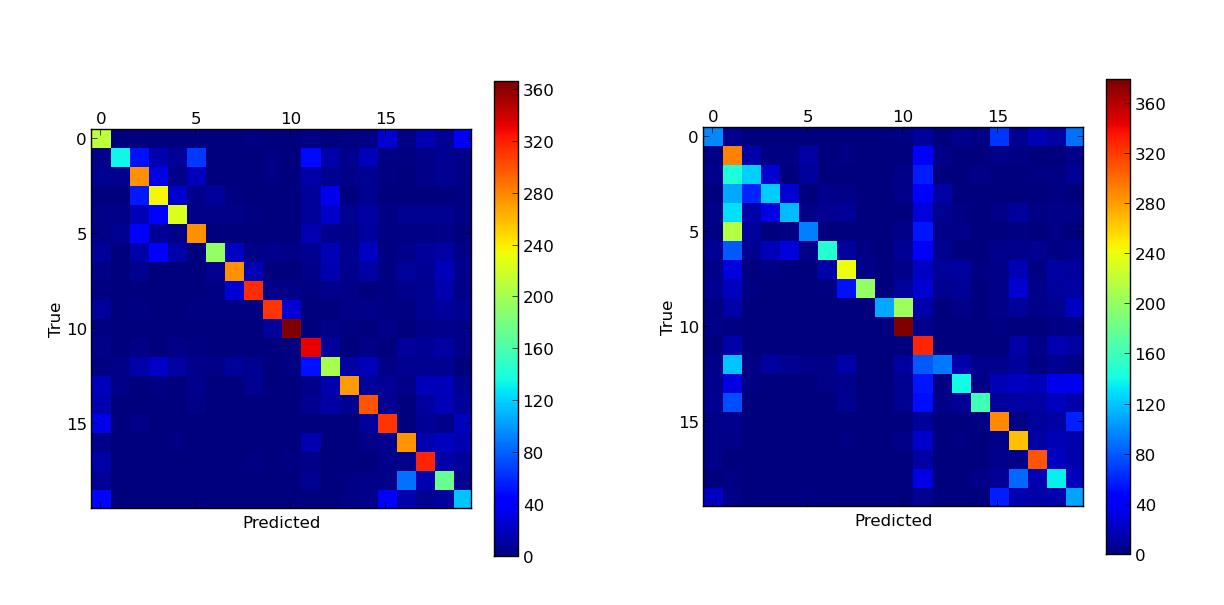
\includegraphics[width=0.45\textwidth]{figures/mnb-conf-1260.png}
    \cprotect\caption{Results for test B: Confusion matrices for best (68.12 \%) 
        and worst (61.99 \%) results of 
        MNB, $|A^\ell| = 1260$.}
    \label{fig:mnb-em-mnb}

\end{figure}

\begin{figure}[h!]

    \centering
    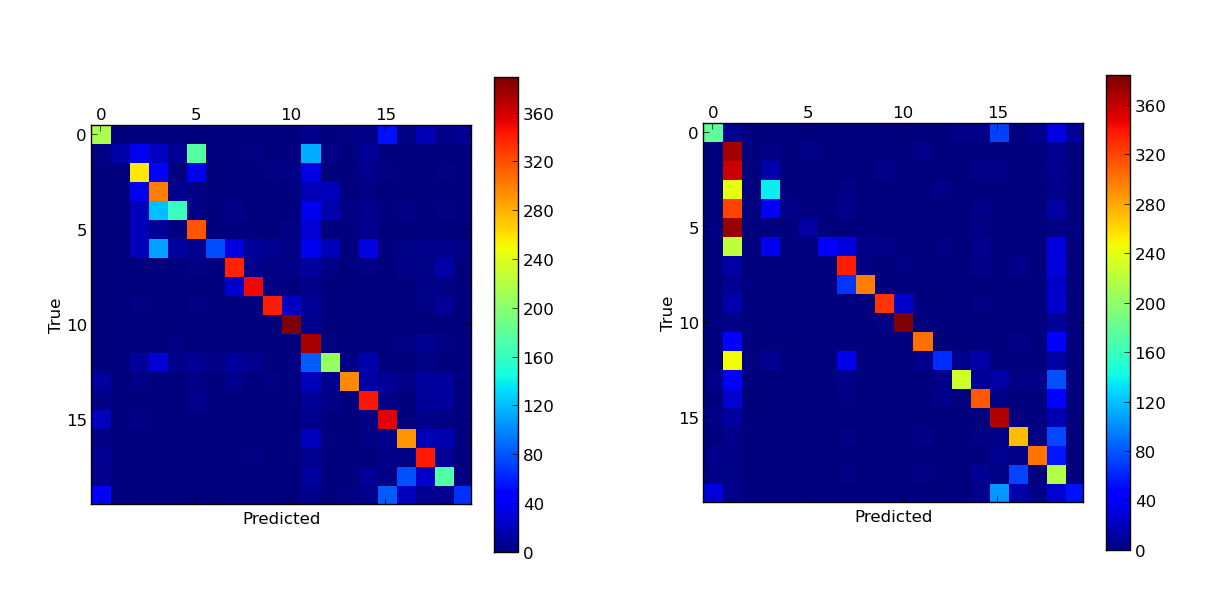
\includegraphics[width=0.45\textwidth]{figures/em-conf-1260.png}
    \cprotect\caption{Results for test B: Confusion matrices for best (left side, 69.44 \%) 
        and worst (right side, 56.04 \%) results of 
        MNB + EM, $|A^\ell| = 1260$.}
    \label{fig:mnb-em-em}

\end{figure}

Figure~\ref{fig:mnb-em-lambda} shows the results for the EM-$\lambda$ method, 
for several values of $L = 1 / \lambda$\,\cprotect\footnote{We use Rainbow's option 
\verb+--em-unlabeled-normalizer+, which determines the number of unlabeled 
articles it takes to equal a labeled article.}. We verified that for low values 
of $|A^\ell|$, lower values of $L$ (and therefore higher $\lambda$) provide 
better results, with the top accuracy verified for $\lambda = 1$. As $|A^\ell|$ 
increases, higher accuracy values tend to be favored by lower values of $\lambda$. 
Nevertheless, the best results for EM-$\lambda$ keep occurring for $\lambda = 1$, 
which seems somewhat counter-intuitive.

\begin{figure}[h!]

    \centering
    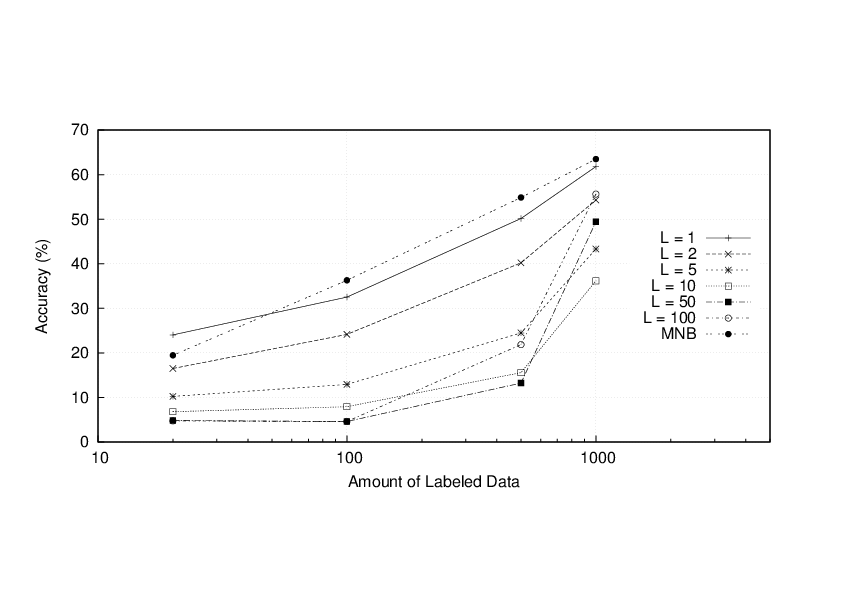
\includegraphics[width=0.40\textwidth]{figures/em-lambda.pdf}
    \cprotect\caption{Results for test C: MNB + EM-$\lambda$, using Rainbow's framework. 
        The results of MNB for the same $A^\ell$ are also given.}
    \label{fig:mnb-em-lambda}

\end{figure}
